\documentclass[14pt]{beamer}
\author{Daniel Wagner}
\usepackage{tikz}
\usepackage{beamer_minimal}
\usepackage{presentation}
\usepackage{amssymb}
\usepackage{semantic}
% TODO: update related work slides on symmetry/edits -- ESPECIALLY edits
\begin{document}

\title{Generalizing Lenses}
\date[University of Pennsylvania]{August 19, 2013}
\begin{frame}
    \maketitle
    \begin{tikzpicture}[remember picture,overlay]
        \node[inner sep=0,outer sep=0,anchor=south east]
            at (current page.south east)
            {\lolcat{peer}}
            ;
    \end{tikzpicture}
\end{frame}

\begin{frame}
    \frametitle{Thesis Proposal}
    \alert<2>{There are many fundamentally bidirectional settings}
    \alert<3>{that call for generalizations of traditional lenses}
    \alert<4>{where a language is possible and helpful.}
\end{frame}

% TODO: make it clear which bits predate me, which bits I helped with, which
% bits are not yet done
\begin{frame}
    \frametitle{Overview}
    \tableofcontents
\end{frame}

\section{Traditional lenses}
\begin{frame}
    \begin{center}
        \begin{tikzpicture}
            \draw[short picture tree]
                node (root) {} child {
                    node (Jan) {Jan\strut}
                        \lolcatchildren{palindrome,gamer}
                } child {
                    node (May) {May\strut}
                        \lolcatchildren{froghead}
                }
                ;
            \lolcatnotagsdef{froghead-fs-pic}
                {palindrome/{costume,food},gamer/{costume},froghead/{costume}}
            \fswebborder{palindrome}{froghead}
        \end{tikzpicture}
    \end{center}
\end{frame}

\begin{frame}
    \begin{center}
        \begin{tikzpicture}
            \draw[short picture tree]
                node (root) {} child {
                    node (Jan) {Jan\strut}
                        \lolcatchildren{palindrome,gamer}
                } child {
                    node (May) {May\strut}
                        \lolcatchildren{froghead}
                }
                ;
            \lolcatnotagsdef{froghead-fs-pic}
                {palindrome/{costume,food},gamer/{costume},froghead/{costume},burrito/{onlyface}}
            \node[fit=(burrito-web-pic)] (burrito-web-alert) {};
            \path[rounded corners,draw=alertgreen]
                ($(burrito-web-alert.north west) +(0.25,-0.25)$) rectangle
                ($(burrito-web-alert.south east) +(-0.25,0.25)$);
            \fsborder{palindrome}{froghead}
            \webborder{palindrome}{burrito}
        \end{tikzpicture}
    \end{center}
\end{frame}

\begin{frame}
    \begin{center}
        \begin{tikzpicture}
            \draw[short picture tree]
                node (root) {} child {
                    node (Jan) {Jan\strut}
                        \lolcatchildren{palindrome,gamer}
                } child {
                    node (May) {May\strut}
                        \lolcatchildren{froghead}
                } child {
                    node        (burrito-fs-name) {\tiny ???}
                    node[below] (burrito-fs-pic)  {\lolcat{burrito}}
                }
                ;
            \lolcatnotagsdef{burrito-fs-pic}
                {palindrome/{costume,food},gamer/{costume},froghead/{costume},burrito/{onlyface}}
            \node[fit=(burrito-fs-pic) (burrito-fs-name)] (burrito-fs-alert) {};
            \path[rounded corners,draw=alertgreen]
                ($(burrito-fs-alert.north west) +(0.25,-0.25)$) rectangle
                ($(burrito-fs-alert.south east) +(-0.25,0.25)$);
            \fswebborder{palindrome}{burrito}
        \end{tikzpicture}
    \end{center}
\end{frame}

\begin{frame}
    \begin{center}
        \begin{tikzpicture}
            \draw[narrow picture tree]
                node (root) {} child {
                    node (Jan) {Jan\strut}
                        \lolcatchildren{palindrome,gamer}
                } child {
                    node (May) {May\strut}
                        \lolcatchildren{froghead}
                } child[sibling distance=1.33cm] {
                    node        (burrito-fs-name) {\tiny burrito.jpg}
                    node[below] (burrito-fs-pic)  {\lolcat{burrito}}
                } child[sibling distance=1.33cm] {
                    node        (withperson-fs-name) {\tiny withperson.jpg}
                    node[below] (withperson-fs-pic)  {\lolcat{withperson}}
                }
                ;
            \node[fit=(withperson-fs-name) (withperson-fs-pic)] (withperson-fs-alert) {};
            \path[rounded corners,draw=alertgreen]
                ($(withperson-fs-alert.north west) +(0.25,-0.25)$) rectangle
                ($(withperson-fs-alert.south east) +(-0.25,0.25)$);
            \lolcatnotags{(root.north -| withperson-fs-pic.east) +(1.3,0)}
                {palindrome/{costume,food},
                 gamer/{costume},
                 froghead/{costume},
                 burrito/{food,onlyface}}
            \fsborder{palindrome}{withperson}
            \webborder{palindrome}{burrito}
        \end{tikzpicture}
    \end{center}
\end{frame}

\begin{frame}
    \begin{center}
        \begin{tikzpicture}
            \draw[narrow picture tree]
                node (root) {} child {
                    node (Jan) {Jan\strut}
                        \lolcatchildren{palindrome,gamer}
                } child {
                    node (May) {May\strut}
                        \lolcatchildren{froghead}
                } child[sibling distance=1.33cm] {
                    node        (burrito-fs-name) {\tiny burrito.jpg}
                    node[below] (burrito-fs-pic)  {\lolcat{burrito}}
                } child[sibling distance=1.33cm] {
                    node        (withperson-fs-name) {\tiny withperson.jpg}
                    node[below] (withperson-fs-pic)  {\lolcat{withperson}}
                }
                ;
            \lolcatnotags{(root.north -| withperson-fs-pic.east) +(1.3,0)}
                {palindrome/{costume,food},
                 gamer/{costume},
                 froghead/{costume},
                 burrito/{food,onlyface},
                 withperson/{\ }}
            \node[fit=(withperson-web-pic)] (withperson-web-alert) {};
            \path[rounded corners,draw=alertgreen]
                ($(withperson-web-alert.north west) +(0.25,-0.25)$) rectangle
                ($(withperson-web-alert.south east) +(-0.25,0.25)$);
             \fswebborder{palindrome}{withperson}
        \end{tikzpicture}
    \end{center}
\end{frame}

\begin{frame}
    % TODO: forgot create!
    \frametitle{Abstract model}
    A lens $\ell \in X \aslens Y$ has components
    \begin{align*}
        get &\in X \to Y \\
        put &\in Y \times X \to X
    \end{align*}
    \pause
    Synchronizing too often doesn't hurt.
    \begin{align*}
        get(put(y,x))&=y \\
        put(get(x),x)&=x \\
        \uncover<3>{\color{gray}put(y',put(y,x))&\color{gray}=put(y',x)}
    \end{align*}
    \uncover<3>{\color{gray}Not synchronizing often enough doesn't hurt.}
\end{frame}

% TODO: check this list of the reams of work on point-free instantiation
% languages to make sure it includes the stuff on strings, relational
% databases, trees, etc.
\begin{frame}
    \frametitle{Related work: asymmetric lenses}
    \begin{itemize}
        \small
        \item Combinators for Bidirectional Tree Transformations

            \quad (Foster, Greenwald, Moore, Pierce, Schmitt;

            \quad POPL 2005)
        \item Relational Lenses: A Language For Updateable Views

            \quad (Bohannon, Vaughn, and Pierce; PODS 2006)
        \item Boomerang: Resourceful Lenses for String Data

            \quad (Bohannon, Foster, Pierce, Pilkiewicz, and Schmitt;

            \quad POPL 2008)

        \item Bidirectional Programming Languages

            \quad (Foster; thesis 2009)
        \item Bidirectionalizing Graph Transformations

            \quad (Hidaka, Hu, Inaba, and Kato; ICFP 2010)
        \item Update Semantics of Relational Views

            \quad (Bancilhon and Spyratos; 1981)
    \end{itemize}
\end{frame}

\collaborators{Martin Hofmann and Benjamin Pierce}
\section{Symmetry}
\begin{frame}
    \begin{center}
        \begin{tikzpicture}
            \draw[narrow picture tree]
                node (root) {} child {
                    node (Jan) {Jan\strut}
                        \lolcatchildren{palindrome,gamer}
                } child {
                    node (May) {May\strut}
                        \lolcatchildren{froghead}
                } child[sibling distance=1.33cm] {
                    node        (burrito-fs-name) {\tiny burrito.jpg}
                    node[below] (burrito-fs-pic)  {\lolcat{burrito}}
                } child[sibling distance=1.33cm] {
                    node        (withperson-fs-name) {\tiny withperson.jpg}
                    node[below] (withperson-fs-pic)  {\lolcat{withperson}}
                }
                ;
            \lolcatnotags{(root.north -| withperson-fs-pic.east) +(1.3,0)}
                {palindrome/{costume,food},
                 gamer/{costume},
                 froghead/{costume},
                 burrito/{food,onlyface},
                 withperson/{\ }}
             \fswebborder{palindrome}{withperson}
        \end{tikzpicture}
    \end{center}
\end{frame}

\begin{frame}
    \begin{center}
        \begin{tikzpicture}
            \draw[narrow picture tree]
                node (root) {} child {
                    node (Jan) {Jan\strut}
                        \lolcatchildren{palindrome,gamer}
                } child {
                    node (May) {May\strut}
                        \lolcatchildren{froghead}
                } child[sibling distance=1.33cm] {
                    node        (burrito-fs-name) {\tiny burrito.jpg}
                    node[below] (burrito-fs-pic)  {\lolcat{burrito}}
                } child[sibling distance=1.33cm] {
                    node        (withperson-fs-name) {\tiny withperson.jpg}
                    node[below] (withperson-fs-pic)  {\lolcat{withperson}}
                }
                ;
            \lolcattags{(root.north -| withperson-fs-pic.east) +(1.3,0)}
                {palindrome/{costume,food},
                 gamer/{costume},
                 froghead/{costume},
                 burrito/{food,onlyface},
                 withperson/{\ }}
             \fswebborder{palindrome}{withperson}
        \end{tikzpicture}
    \end{center}
\end{frame}

\begin{frame}
    \begin{center}
        \begin{tikzpicture}
            \draw[narrow picture tree]
                node (root) {} child {
                    node (Jan) {Jan\strut} child {
                        node        (palindrome-fs-name) {\tiny palindrome.jpg}
                        node[below] (palindrome-fs-tag)  {\tiny [costume,food]} (palindrome-fs-tag)
                        node[below] (palindrome-fs-pic)  {\lolcat{palindrome}}
                    } child {
                        node        (gamer-fs-name) {\tiny gamer.jpg}
                        node[below] (gamer-fs-tag)  {\tiny [costume]} (gamer-fs-tag)
                        node[below] (gamer-fs-pic)  {\lolcat{gamer}}
                    }
                } child {
                    node (May) {May\strut} child {
                        node        (froghead-fs-name) {\tiny froghead.jpg}
                        node[below] (froghead-fs-tag)  {\tiny [costume]} (froghead-fs-tag)
                        node[below] (froghead-fs-pic)  {\lolcat{froghead}}
                    }
                } child[sibling distance=1.33cm] {
                    node        (burrito-fs-name) {\tiny burrito.jpg}
                    node[below] (burrito-fs-tag)  {\tiny [food,onlyface]} (burrito-fs-tag)
                    node[below] (burrito-fs-pic)  {\lolcat{burrito}}
                } child[sibling distance=1.33cm] {
                    node        (withperson-fs-name) {\tiny withperson.jpg}
                    node[below] (withperson-fs-tag)  {\tiny [\ ]} (withperson-fs-tag)
                    node[below] (withperson-fs-pic)  {\lolcat{withperson}}
                }
                ;
            \lolcattags{(root.north -| withperson-fs-pic.east) +(1.3,0)}
                {palindrome/{costume,food},
                 gamer/{costume},
                 froghead/{costume},
                 burrito/{food,onlyface},
                 withperson/{\ }}
             \fswebborder{palindrome}{withperson}
             \path[use as bounding box] (fs.north west) -- (web.south east);
             \draw<2>[line width=0.6cm,red!70!black] (fs.center)
                circle (3.2cm)
                +(135:3.2cm) -- +(315:3.2cm)
                ;
        \end{tikzpicture}
    \end{center}
\end{frame}

\begin{frame}
    \begin{center}
        \begin{tikzpicture}
            \draw[narrow picture tree]
                node (root) {} child {
                    node (Jan) {Jan\strut}
                        \lolcatchildren{palindrome,gamer}
                } child {
                    node (May) {May\strut}
                        \lolcatchildren{froghead}
                } child[sibling distance=1.33cm] {
                    node        (burrito-fs-name) {\tiny burrito.jpg}
                    node[below] (burrito-fs-pic)  {\lolcat{burrito}}
                } child[sibling distance=1.33cm] {
                    node        (withperson-fs-name) {\tiny withperson.jpg}
                    node[below] (withperson-fs-pic)  {\lolcat{withperson}}
                }
                ;
            \lolcattags{(root.north -| withperson-fs-pic.east) +(1.3,0)}
                {palindrome/{costume,food},
                 gamer/{costume},
                 froghead/{costume},
                 burrito/{food,onlyface},
                 withperson/{\ }}
             \fswebborder{palindrome}{withperson}
             \path[tiny complement tree] (fs.south) ++(-0.8cm, -0.6cm)
                node (complement-root) {} child {
                    node (complement-Jan) {Jan\strut} child {
                        node (complement-palindrome) {palindrome\strut}
                    } child {
                        node (complement-gamer) {gamer\strut}
                    }
                } child {
                    node (complement-May) {May\strut} child {
                        node (complement-froghead) {froghead\strut}
                    }
                } child {
                    node (complement-burrito) {burrito\strut}
                } child {
                    node (complement-withperson) {withperson\strut}
                }
                ;
                \begin{scope}[start chain=going below,node distance=0,inner sep=0.2ex,font=\tiny]
                    \path (complement-root) ++(3.5cm,-0.1cm)
                        node[on chain] (complement-palindrome-tag) {[costume,food]}
                        node[on chain] (complement-gamer-tag)      {[costume]}
                        node[on chain] (complement-froghead-tag)   {[costume]}
                        node[on chain] (complement-burrito-tag)    {[food,onlyface]}
                        node[on chain] (complement-withperson-tag) {[\ ]}
                        ;
                \end{scope}
                \uncover<2>{\path
                    node[fit=(complement-root)
                             (complement-palindrome)
                             (complement-palindrome-tag)
                             (complement-withperson-tag)] (complement) {}
                    (complement) node[anchor=center,scale=3] (complement-check)
                        {\Large\color{alertgreen}\checkmark}
                    ;
                }
        \end{tikzpicture}
    \end{center}
\end{frame}

\begin{frame}
    \frametitle{Abstract model}
    A lens $\ell \in X \sslens Y$ has a set $C$ and components
    \begin{align*}
        putr &\in X\times C \to Y\times C \\
        putl &\in Y\times C \to X\times C
    \end{align*}
    \pause
    Synchronizing too often doesn't hurt.
    \[\inference{putr(x,c)=(y,c')}{putl(y,c')=(x,c')}\]
    \pause
    \color{gray}Not synchronizing often enough doesn't hurt.
    \[putr(x,c)=putr(x,c')\]
\end{frame}

\begin{frame}
    \frametitle{Twist: equational reasoning}
    \begin{center}
        \begin{tikzpicture}[start chain=going right]
            \path
                node[on chain] (A) {A}
                node[on chain] (B) {B}
                node[on chain] (C) {C}
                node[on chain] (D) {D}
                ;
            \draw[<->] (A) -- node[above] {\tiny$a$} node[below] {$k$}    (B);
            \draw[<->] (B) -- node[above] {\tiny$a$} node[below] {$\ell$} (C);
            \draw[<->] (C) -- node[above] {\tiny$a$} node[below] {$m$}    (D);
        \end{tikzpicture}
    \end{center}
    Nice property of asymmetric lenses:
    \[(k;\ell);m = k;(\ell;m)\]
    \pause
    \alert{Not true for symmetric lenses!}
\end{frame}

\begin{frame}
    \frametitle{In dissertation}
    \begin{itemize}
        \item Observational equivalence
        \item Point-free programming language
            \begin{itemize}
                \item Basic (non-recursive) data types
                \item Lists, with folds and unfolds
                \item Some generalized container operations
            \end{itemize}
        \item Proof that this generalizes asymmetric lenses
    \end{itemize}
\end{frame}

\begin{frame}
    \frametitle{Related work: other symmetric approaches}
    \begin{itemize}
        \small
        \item Symmetric Constraint Maintainers

            \quad (Meertens; 1998)
        \item Towards an Algebraic Theory of Bidirectional Transformations

            \quad (Stevens; ICGT 2008)
        \item Bidirectional Model Transformations in QVT: Semantic Issues
            and Open Questions

            \quad (Stevens; MoDELS 2007)
        \item Algebraic Models for Bidirectional Model Synchronization

            \quad (Diskin; MoDELS 2008)

        \item Supporting Parallel Updates with Bidirectional Model
            Transformations

            \quad (Xiong, Song, Hu, and Takeichi; ICMT 2009)
    \end{itemize}
\end{frame}

\collaborators{Martin Hofmann and Benjamin Pierce}
\section{Edits}
\begin{frame}
    \begin{center}
        \begin{tikzpicture}
            \draw[narrow picture tree]
                node (root) {} child {
                    node (Jan) {Jan\strut}
                        \lolcatchildren{palindrome,gamer}
                } child {
                    node (May) {May\strut}
                        \lolcatchildren{froghead}
                } child[sibling distance=1.33cm] {
                    node        (burrito-fs-name) {\tiny burrito.jpg}
                    node[below] (burrito-fs-pic)  {\lolcat{burrito}}
                } child[sibling distance=1.33cm] {
                    node        (withperson-fs-name) {\tiny withperson.jpg}
                    node[below] (withperson-fs-pic)  {\lolcat{withperson}}
                }
                ;
            \lolcattags{(root.north -| withperson-fs-pic.east) +(1.3,0)}
                {palindrome/{costume,food},
                 gamer/{costume},
                 froghead/{costume},
                 burrito/{food,onlyface},
                 withperson/{\ }}
             \fswebborder{palindrome}{withperson}
        \end{tikzpicture}
    \end{center}
\end{frame}

\begin{frame}
    \begin{center}
        \begin{tikzpicture}
% generated by random_cats.hs
\draw[busy picture tree] node (root) {}child{node[inner sep=0,scale=0.5](2012){\strut 2012}child{node[inner sep=0,scale=0.1](January){\strut January}child{node[scale=0.1](first-fs-name){\tiny wrapped.jpg}node[below,scale=0.05](first-fs-pic){\lolcat{wrapped}}}child{node[scale=0.1](last-fs-name){\tiny gamer.jpg}node[below,scale=0.05](last-fs-pic){\lolcat{gamer}}}child{node[scale=0.1](last-fs-name){\tiny froghead.jpg}node[below,scale=0.05](last-fs-pic){\lolcat{froghead}}}}child{node[inner sep=0,scale=0.1](February){\strut February}child{node[scale=0.1](last-fs-name){\tiny wrapped.jpg}node[below,scale=0.05](last-fs-pic){\lolcat{wrapped}}}child{node[scale=0.1](last-fs-name){\tiny burrito.jpg}node[below,scale=0.05](last-fs-pic){\lolcat{burrito}}}child{node[scale=0.1](last-fs-name){\tiny gamer.jpg}node[below,scale=0.05](last-fs-pic){\lolcat{gamer}}}}child{node[inner sep=0,scale=0.1](March){\strut March}child{node[scale=0.1](last-fs-name){\tiny palindrome.jpg}node[below,scale=0.05](last-fs-pic){\lolcat{palindrome}}}child{node[scale=0.1](last-fs-name){\tiny gamer.jpg}node[below,scale=0.05](last-fs-pic){\lolcat{gamer}}}child{node[scale=0.1](last-fs-name){\tiny dune.jpg}node[below,scale=0.05](last-fs-pic){\lolcat{dune}}}child{node[scale=0.1](last-fs-name){\tiny palindrome.jpg}node[below,scale=0.05](last-fs-pic){\lolcat{palindrome}}}child{node[scale=0.1](last-fs-name){\tiny dune.jpg}node[below,scale=0.05](last-fs-pic){\lolcat{dune}}}}child{node[inner sep=0,scale=0.1](April){\strut April}child{node[scale=0.1](last-fs-name){\tiny palindrome.jpg}node[below,scale=0.05](last-fs-pic){\lolcat{palindrome}}}child{node[scale=0.1](last-fs-name){\tiny lobster.jpg}node[below,scale=0.05](last-fs-pic){\lolcat{lobster}}}child{node[scale=0.1](last-fs-name){\tiny withperson.jpg}node[below,scale=0.05](last-fs-pic){\lolcat{withperson}}}}child{node[inner sep=0,scale=0.1](May){\strut May}child{node[scale=0.1](last-fs-name){\tiny wrapped.jpg}node[below,scale=0.05](last-fs-pic){\lolcat{wrapped}}}child{node[scale=0.1](last-fs-name){\tiny dune.jpg}node[below,scale=0.05](last-fs-pic){\lolcat{dune}}}child{node[scale=0.1](last-fs-name){\tiny froghead.jpg}node[below,scale=0.05](last-fs-pic){\lolcat{froghead}}}child{node[scale=0.1](last-fs-name){\tiny dune.jpg}node[below,scale=0.05](last-fs-pic){\lolcat{dune}}}}child{node[inner sep=0,scale=0.1](June){\strut June}child{node[scale=0.1](last-fs-name){\tiny burrito.jpg}node[below,scale=0.05](last-fs-pic){\lolcat{burrito}}}child{node[scale=0.1](last-fs-name){\tiny froghead.jpg}node[below,scale=0.05](last-fs-pic){\lolcat{froghead}}}child{node[scale=0.1](last-fs-name){\tiny gamer.jpg}node[below,scale=0.05](last-fs-pic){\lolcat{gamer}}}child{node[scale=0.1](last-fs-name){\tiny dune.jpg}node[below,scale=0.05](last-fs-pic){\lolcat{dune}}}}child{node[inner sep=0,scale=0.1](July){\strut July}child{node[scale=0.1](last-fs-name){\tiny gamer.jpg}node[below,scale=0.05](last-fs-pic){\lolcat{gamer}}}child{node[scale=0.1](last-fs-name){\tiny froghead.jpg}node[below,scale=0.05](last-fs-pic){\lolcat{froghead}}}child{node[scale=0.1](last-fs-name){\tiny withperson.jpg}node[below,scale=0.05](last-fs-pic){\lolcat{withperson}}}}child{node[inner sep=0,scale=0.1](August){\strut August}child{node[scale=0.1](last-fs-name){\tiny burrito.jpg}node[below,scale=0.05](last-fs-pic){\lolcat{burrito}}}child{node[scale=0.1](last-fs-name){\tiny froghead.jpg}node[below,scale=0.05](last-fs-pic){\lolcat{froghead}}}child{node[scale=0.1](last-fs-name){\tiny dune.jpg}node[below,scale=0.05](last-fs-pic){\lolcat{dune}}}child{node[scale=0.1](last-fs-name){\tiny froghead.jpg}node[below,scale=0.05](last-fs-pic){\lolcat{froghead}}}}child{node[inner sep=0,scale=0.1](September){\strut September}child{node[scale=0.1](last-fs-name){\tiny palindrome.jpg}node[below,scale=0.05](last-fs-pic){\lolcat{palindrome}}}child{node[scale=0.1](last-fs-name){\tiny lobster.jpg}node[below,scale=0.05](last-fs-pic){\lolcat{lobster}}}child{node[scale=0.1](last-fs-name){\tiny gamer.jpg}node[below,scale=0.05](last-fs-pic){\lolcat{gamer}}}}child{node[inner sep=0,scale=0.1](October){\strut October}child{node[scale=0.1](last-fs-name){\tiny withperson.jpg}node[below,scale=0.05](last-fs-pic){\lolcat{withperson}}}child{node[scale=0.1](last-fs-name){\tiny palindrome.jpg}node[below,scale=0.05](last-fs-pic){\lolcat{palindrome}}}child{node[scale=0.1](last-fs-name){\tiny gamer.jpg}node[below,scale=0.05](last-fs-pic){\lolcat{gamer}}}}child{node[inner sep=0,scale=0.1](November){\strut November}child{node[scale=0.1](last-fs-name){\tiny froghead.jpg}node[below,scale=0.05](last-fs-pic){\lolcat{froghead}}}child{node[scale=0.1](last-fs-name){\tiny burrito.jpg}node[below,scale=0.05](last-fs-pic){\lolcat{burrito}}}child{node[scale=0.1](last-fs-name){\tiny gamer.jpg}node[below,scale=0.05](last-fs-pic){\lolcat{gamer}}}child{node[scale=0.1](last-fs-name){\tiny burrito.jpg}node[below,scale=0.05](last-fs-pic){\lolcat{burrito}}}child{node[scale=0.1](last-fs-name){\tiny withperson.jpg}node[below,scale=0.05](last-fs-pic){\lolcat{withperson}}}}child{node[inner sep=0,scale=0.1](December){\strut December}child{node[scale=0.1](last-fs-name){\tiny gamer.jpg}node[below,scale=0.05](last-fs-pic){\lolcat{gamer}}}child{node[scale=0.1](last-fs-name){\tiny wrapped.jpg}node[below,scale=0.05](last-fs-pic){\lolcat{wrapped}}}child{node[scale=0.1](last-fs-name){\tiny dune.jpg}node[below,scale=0.05](last-fs-pic){\lolcat{dune}}}child{node[scale=0.1](last-fs-name){\tiny lobster.jpg}node[below,scale=0.05](last-fs-pic){\lolcat{lobster}}}}}child{node[inner sep=0,scale=0.5](2013){\strut 2013}child{node[inner sep=0,scale=0.1](January){\strut January}child{node[scale=0.1](last-fs-name){\tiny froghead.jpg}node[below,scale=0.05](last-fs-pic){\lolcat{froghead}}}child{node[scale=0.1](last-fs-name){\tiny withperson.jpg}node[below,scale=0.05](last-fs-pic){\lolcat{withperson}}}child{node[scale=0.1](last-fs-name){\tiny palindrome.jpg}node[below,scale=0.05](last-fs-pic){\lolcat{palindrome}}}child{node[scale=0.1](last-fs-name){\tiny wrapped.jpg}node[below,scale=0.05](last-fs-pic){\lolcat{wrapped}}}}child{node[inner sep=0,scale=0.1](February){\strut February}child{node[scale=0.1](last-fs-name){\tiny dune.jpg}node[below,scale=0.05](last-fs-pic){\lolcat{dune}}}child{node[scale=0.1](last-fs-name){\tiny froghead.jpg}node[below,scale=0.05](last-fs-pic){\lolcat{froghead}}}child{node[scale=0.1](last-fs-name){\tiny palindrome.jpg}node[below,scale=0.05](last-fs-pic){\lolcat{palindrome}}}}child{node[inner sep=0,scale=0.1](March){\strut March}child{node[scale=0.1](last-fs-name){\tiny lobster.jpg}node[below,scale=0.05](last-fs-pic){\lolcat{lobster}}}child{node[scale=0.1](last-fs-name){\tiny froghead.jpg}node[below,scale=0.05](last-fs-pic){\lolcat{froghead}}}child{node[scale=0.1](last-fs-name){\tiny palindrome.jpg}node[below,scale=0.05](last-fs-pic){\lolcat{palindrome}}}}child{node[inner sep=0,scale=0.1](April){\strut April}child{node[scale=0.1](last-fs-name){\tiny dune.jpg}node[below,scale=0.05](last-fs-pic){\lolcat{dune}}}child{node[scale=0.1](last-fs-name){\tiny gamer.jpg}node[below,scale=0.05](last-fs-pic){\lolcat{gamer}}}child{node[scale=0.1](last-fs-name){\tiny withperson.jpg}node[below,scale=0.05](last-fs-pic){\lolcat{withperson}}}child{node[scale=0.1](last-fs-name){\tiny dune.jpg}node[below,scale=0.05](last-fs-pic){\lolcat{dune}}}child{node[scale=0.1](last-fs-name){\tiny wrapped.jpg}node[below,scale=0.05](last-fs-pic){\lolcat{wrapped}}}}child{node[inner sep=0,scale=0.1](May){\strut May}child{node[scale=0.1](last-fs-name){\tiny withperson.jpg}node[below,scale=0.05](last-fs-pic){\lolcat{withperson}}}child{node[scale=0.1](last-fs-name){\tiny burrito.jpg}node[below,scale=0.05](last-fs-pic){\lolcat{burrito}}}child{node[scale=0.1](last-fs-name){\tiny withperson.jpg}node[below,scale=0.05](last-fs-pic){\lolcat{withperson}}}child{node[scale=0.1](last-fs-name){\tiny froghead.jpg}node[below,scale=0.05](last-fs-pic){\lolcat{froghead}}}child{node[scale=0.1](last-fs-name){\tiny lobster.jpg}node[below,scale=0.05](last-fs-pic){\lolcat{lobster}}}}child{node[inner sep=0,scale=0.1](June){\strut June}child{node[scale=0.1](last-fs-name){\tiny wrapped.jpg}node[below,scale=0.05](last-fs-pic){\lolcat{wrapped}}}child{node[scale=0.1](last-fs-name){\tiny burrito.jpg}node[below,scale=0.05](last-fs-pic){\lolcat{burrito}}}child{node[scale=0.1](last-fs-name){\tiny wrapped.jpg}node[below,scale=0.05](last-fs-pic){\lolcat{wrapped}}}child{node[scale=0.1](last-fs-name){\tiny palindrome.jpg}node[below,scale=0.05](last-fs-pic){\lolcat{palindrome}}}child{node[scale=0.1](last-fs-name){\tiny burrito.jpg}node[below,scale=0.05](last-fs-pic){\lolcat{burrito}}}}child{node[inner sep=0,scale=0.1](July){\strut July}child{node[scale=0.1](last-fs-name){\tiny palindrome.jpg}node[below,scale=0.05](last-fs-pic){\lolcat{palindrome}}}child{node[scale=0.1](last-fs-name){\tiny withperson.jpg}node[below,scale=0.05](last-fs-pic){\lolcat{withperson}}}child{node[scale=0.1](last-fs-name){\tiny burrito.jpg}node[below,scale=0.05](last-fs-pic){\lolcat{burrito}}}child{node[scale=0.1](last-fs-name){\tiny wrapped.jpg}node[below,scale=0.05](last-fs-pic){\lolcat{wrapped}}}}child{node[inner sep=0,scale=0.1](August){\strut August}child{node[scale=0.1](last-fs-name){\tiny gamer.jpg}node[below,scale=0.05](last-fs-pic){\lolcat{gamer}}}child{node[scale=0.1](last-fs-name){\tiny froghead.jpg}node[below,scale=0.05](last-fs-pic){\lolcat{froghead}}}child{node[scale=0.1](last-fs-name){\tiny wrapped.jpg}node[below,scale=0.05](last-fs-pic){\lolcat{wrapped}}}child{node[scale=0.1](last-fs-name){\tiny withperson.jpg}node[below,scale=0.05](last-fs-pic){\lolcat{withperson}}}child{node[scale=0.1](last-fs-name){\tiny gamer.jpg}node[below,scale=0.05](last-fs-pic){\lolcat{gamer}}}}child{node[inner sep=0,scale=0.1](September){\strut September}child{node[scale=0.1](last-fs-name){\tiny froghead.jpg}node[below,scale=0.05](last-fs-pic){\lolcat{froghead}}}child{node[scale=0.1](last-fs-name){\tiny lobster.jpg}node[below,scale=0.05](last-fs-pic){\lolcat{lobster}}}child{node[scale=0.1](last-fs-name){\tiny palindrome.jpg}node[below,scale=0.05](last-fs-pic){\lolcat{palindrome}}}child{node[scale=0.1](last-fs-name){\tiny gamer.jpg}node[below,scale=0.05](last-fs-pic){\lolcat{gamer}}}child{node[scale=0.1](last-fs-name){\tiny burrito.jpg}node[below,scale=0.05](last-fs-pic){\lolcat{burrito}}}}child{node[inner sep=0,scale=0.1](October){\strut October}child{node[scale=0.1](last-fs-name){\tiny froghead.jpg}node[below,scale=0.05](last-fs-pic){\lolcat{froghead}}}child{node[scale=0.1](last-fs-name){\tiny withperson.jpg}node[below,scale=0.05](last-fs-pic){\lolcat{withperson}}}child{node[scale=0.1](last-fs-name){\tiny dune.jpg}node[below,scale=0.05](last-fs-pic){\lolcat{dune}}}}child{node[inner sep=0,scale=0.1](November){\strut November}child{node[scale=0.1](last-fs-name){\tiny burrito.jpg}node[below,scale=0.05](last-fs-pic){\lolcat{burrito}}}child{node[scale=0.1](last-fs-name){\tiny withperson.jpg}node[below,scale=0.05](last-fs-pic){\lolcat{withperson}}}child{node[scale=0.1](last-fs-name){\tiny wrapped.jpg}node[below,scale=0.05](last-fs-pic){\lolcat{wrapped}}}}child{node[inner sep=0,scale=0.1](December){\strut December}child{node[scale=0.1](last-fs-name){\tiny froghead.jpg}node[below,scale=0.05](last-fs-pic){\lolcat{froghead}}}child{node[scale=0.1](last-fs-name){\tiny burrito.jpg}node[below,scale=0.05](last-fs-pic){\lolcat{burrito}}}child{node[scale=0.1](last-fs-name){\tiny froghead.jpg}node[below,scale=0.05](last-fs-pic){\lolcat{froghead}}}}};\fsborder{first}{last}\begin{scope}[start chain=going below,node distance=0]\draw(root.north -| last-fs-pic.east) +(1.3,0)node[on chain,anchor=north,scale=0.06](first-web-pic){\lolcat{wrapped}}node[right=of first-web-pic,scale=0.06](first-web-tag){\tiny [cute]}node[on chain,anchor=north,scale=0.06](last-web-pic){\lolcat{gamer}}node[right=of last-web-pic,scale=0.06](last-web-tag){\tiny [kitten,invisible,apathy]}node[on chain,anchor=north,scale=0.06](last-web-pic){\lolcat{froghead}}node[right=of last-web-pic,scale=0.06](last-web-tag){\tiny [food,costume,cute]}node[on chain,anchor=north,scale=0.06](last-web-pic){\lolcat{wrapped}}node[right=of last-web-pic,scale=0.06](last-web-tag){\tiny [food]}node[on chain,anchor=north,scale=0.06](last-web-pic){\lolcat{burrito}}node[right=of last-web-pic,scale=0.06](last-web-tag){\tiny [costume]}node[on chain,anchor=north,scale=0.06](last-web-pic){\lolcat{gamer}}node[right=of last-web-pic,scale=0.06](last-web-tag){\tiny [dog,kitten]}node[on chain,anchor=north,scale=0.06](last-web-pic){\lolcat{palindrome}}node[right=of last-web-pic,scale=0.06](last-web-tag){\tiny [food]}node[on chain,anchor=north,scale=0.06](last-web-pic){\lolcat{gamer}}node[right=of last-web-pic,scale=0.06](last-web-tag){\tiny [invisible,food]}node[on chain,anchor=north,scale=0.06](last-web-pic){\lolcat{dune}}node[right=of last-web-pic,scale=0.06](last-web-tag){\tiny [food,cute]}node[on chain,anchor=north,scale=0.06](last-web-pic){\lolcat{palindrome}}node[right=of last-web-pic,scale=0.06](last-web-tag){\tiny [food,cute]}node[on chain,anchor=north,scale=0.06](last-web-pic){\lolcat{dune}}node[right=of last-web-pic,scale=0.06](last-web-tag){\tiny [\ ]}node[on chain,anchor=north,scale=0.06](last-web-pic){\lolcat{palindrome}}node[right=of last-web-pic,scale=0.06](last-web-tag){\tiny [\ ]}node[on chain,anchor=north,scale=0.06](last-web-pic){\lolcat{lobster}}node[right=of last-web-pic,scale=0.06](last-web-tag){\tiny [costume,dog]}node[on chain,anchor=north,scale=0.06](last-web-pic){\lolcat{withperson}}node[right=of last-web-pic,scale=0.06](last-web-tag){\tiny [dog,kitten,invisible]}node[on chain,anchor=north,scale=0.06](last-web-pic){\lolcat{wrapped}}node[right=of last-web-pic,scale=0.06](last-web-tag){\tiny [\ ]}node[on chain,anchor=north,scale=0.06](last-web-pic){\lolcat{dune}}node[right=of last-web-pic,scale=0.06](last-web-tag){\tiny [\ ]}node[on chain,anchor=north,scale=0.06](last-web-pic){\lolcat{froghead}}node[right=of last-web-pic,scale=0.06](last-web-tag){\tiny [\ ]}node[on chain,anchor=north,scale=0.06](last-web-pic){\lolcat{dune}}node[right=of last-web-pic,scale=0.06](last-web-tag){\tiny [\ ]}node[on chain,anchor=north,scale=0.06](last-web-pic){\lolcat{burrito}}node[right=of last-web-pic,scale=0.06](last-web-tag){\tiny [\ ]}node[on chain,anchor=north,scale=0.06](last-web-pic){\lolcat{froghead}}node[right=of last-web-pic,scale=0.06](last-web-tag){\tiny [food,dog]}node[on chain,anchor=north,scale=0.06](last-web-pic){\lolcat{gamer}}node[right=of last-web-pic,scale=0.06](last-web-tag){\tiny [\ ]}node[on chain,anchor=north,scale=0.06](last-web-pic){\lolcat{dune}}node[right=of last-web-pic,scale=0.06](last-web-tag){\tiny [kitten]}node[on chain,anchor=north,scale=0.06](last-web-pic){\lolcat{gamer}}node[right=of last-web-pic,scale=0.06](last-web-tag){\tiny [\ ]}node[on chain,anchor=north,scale=0.06](last-web-pic){\lolcat{froghead}}node[right=of last-web-pic,scale=0.06](last-web-tag){\tiny [\ ]}node[on chain,anchor=north,scale=0.06](last-web-pic){\lolcat{withperson}}node[right=of last-web-pic,scale=0.06](last-web-tag){\tiny [invisible,cute,costume]}node[on chain,anchor=north,scale=0.06](last-web-pic){\lolcat{burrito}}node[right=of last-web-pic,scale=0.06](last-web-tag){\tiny [\ ]}node[on chain,anchor=north,scale=0.06](last-web-pic){\lolcat{froghead}}node[right=of last-web-pic,scale=0.06](last-web-tag){\tiny [\ ]}node[on chain,anchor=north,scale=0.06](last-web-pic){\lolcat{dune}}node[right=of last-web-pic,scale=0.06](last-web-tag){\tiny [food,invisible]}node[on chain,anchor=north,scale=0.06](last-web-pic){\lolcat{froghead}}node[right=of last-web-pic,scale=0.06](last-web-tag){\tiny [kitten,dog]}node[on chain,anchor=north,scale=0.06](last-web-pic){\lolcat{palindrome}}node[right=of last-web-pic,scale=0.06](last-web-tag){\tiny [invisible,kitten]}node[on chain,anchor=north,scale=0.06](last-web-pic){\lolcat{lobster}}node[right=of last-web-pic,scale=0.06](last-web-tag){\tiny [costume,cute,onlyface]}node[on chain,anchor=north,scale=0.06](last-web-pic){\lolcat{gamer}}node[right=of last-web-pic,scale=0.06](last-web-tag){\tiny [cute]}node[on chain,anchor=north,scale=0.06](last-web-pic){\lolcat{withperson}}node[right=of last-web-pic,scale=0.06](last-web-tag){\tiny [\ ]}node[on chain,anchor=north,scale=0.06](last-web-pic){\lolcat{palindrome}}node[right=of last-web-pic,scale=0.06](last-web-tag){\tiny [\ ]}node[on chain,anchor=north,scale=0.06](last-web-pic){\lolcat{gamer}}node[right=of last-web-pic,scale=0.06](last-web-tag){\tiny [onlyface]}node[on chain,anchor=north,scale=0.06](last-web-pic){\lolcat{froghead}}node[right=of last-web-pic,scale=0.06](last-web-tag){\tiny [invisible,onlyface]}node[on chain,anchor=north,scale=0.06](last-web-pic){\lolcat{burrito}}node[right=of last-web-pic,scale=0.06](last-web-tag){\tiny [\ ]}node[on chain,anchor=north,scale=0.06](last-web-pic){\lolcat{gamer}}node[right=of last-web-pic,scale=0.06](last-web-tag){\tiny [\ ]}node[on chain,anchor=north,scale=0.06](last-web-pic){\lolcat{burrito}}node[right=of last-web-pic,scale=0.06](last-web-tag){\tiny [cute]}node[on chain,anchor=north,scale=0.06](last-web-pic){\lolcat{withperson}}node[right=of last-web-pic,scale=0.06](last-web-tag){\tiny [\ ]}node[on chain,anchor=north,scale=0.06](last-web-pic){\lolcat{gamer}}node[right=of last-web-pic,scale=0.06](last-web-tag){\tiny [dog,cute]}node[on chain,anchor=north,scale=0.06](last-web-pic){\lolcat{wrapped}}node[right=of last-web-pic,scale=0.06](last-web-tag){\tiny [\ ]}node[on chain,anchor=north,scale=0.06](last-web-pic){\lolcat{dune}}node[right=of last-web-pic,scale=0.06](last-web-tag){\tiny [costume]}node[on chain,anchor=north,scale=0.06](last-web-pic){\lolcat{lobster}}node[right=of last-web-pic,scale=0.06](last-web-tag){\tiny [\ ]}node[on chain,anchor=north,scale=0.06](last-web-pic){\lolcat{froghead}}node[right=of last-web-pic,scale=0.06](last-web-tag){\tiny [\ ]}node[on chain,anchor=north,scale=0.06](last-web-pic){\lolcat{withperson}}node[right=of last-web-pic,scale=0.06](last-web-tag){\tiny [\ ]}node[on chain,anchor=north,scale=0.06](last-web-pic){\lolcat{palindrome}}node[right=of last-web-pic,scale=0.06](last-web-tag){\tiny [kitten,apathy,cute]}node[on chain,anchor=north,scale=0.06](last-web-pic){\lolcat{wrapped}}node[right=of last-web-pic,scale=0.06](last-web-tag){\tiny [\ ]}node[on chain,anchor=north,scale=0.06](last-web-pic){\lolcat{dune}}node[right=of last-web-pic,scale=0.06](last-web-tag){\tiny [onlyface]}node[on chain,anchor=north,scale=0.06](last-web-pic){\lolcat{froghead}}node[right=of last-web-pic,scale=0.06](last-web-tag){\tiny [\ ]}node[on chain,anchor=north,scale=0.06](last-web-pic){\lolcat{palindrome}}node[right=of last-web-pic,scale=0.06](last-web-tag){\tiny [food,cute,invisible]}node[on chain,anchor=north,scale=0.06](last-web-pic){\lolcat{lobster}}node[right=of last-web-pic,scale=0.06](last-web-tag){\tiny [invisible,apathy,costume]}node[on chain,anchor=north,scale=0.06](last-web-pic){\lolcat{froghead}}node[right=of last-web-pic,scale=0.06](last-web-tag){\tiny [dog]}node[on chain,anchor=north,scale=0.06](last-web-pic){\lolcat{palindrome}}node[right=of last-web-pic,scale=0.06](last-web-tag){\tiny [costume,dog]}node[on chain,anchor=north,scale=0.06](last-web-pic){\lolcat{dune}}node[right=of last-web-pic,scale=0.06](last-web-tag){\tiny [\ ]}node[on chain,anchor=north,scale=0.06](last-web-pic){\lolcat{gamer}}node[right=of last-web-pic,scale=0.06](last-web-tag){\tiny [dog]}node[on chain,anchor=north,scale=0.06](last-web-pic){\lolcat{withperson}}node[right=of last-web-pic,scale=0.06](last-web-tag){\tiny [apathy]}node[on chain,anchor=north,scale=0.06](last-web-pic){\lolcat{dune}}node[right=of last-web-pic,scale=0.06](last-web-tag){\tiny [onlyface]}node[on chain,anchor=north,scale=0.06](last-web-pic){\lolcat{wrapped}}node[right=of last-web-pic,scale=0.06](last-web-tag){\tiny [kitten]}node[on chain,anchor=north,scale=0.06](last-web-pic){\lolcat{withperson}}node[right=of last-web-pic,scale=0.06](last-web-tag){\tiny [costume,apathy]}node[on chain,anchor=north,scale=0.06](last-web-pic){\lolcat{burrito}}node[right=of last-web-pic,scale=0.06](last-web-tag){\tiny [invisible,onlyface]}node[on chain,anchor=north,scale=0.06](last-web-pic){\lolcat{withperson}}node[right=of last-web-pic,scale=0.06](last-web-tag){\tiny [kitten,onlyface,apathy]}node[on chain,anchor=north,scale=0.06](last-web-pic){\lolcat{froghead}}node[right=of last-web-pic,scale=0.06](last-web-tag){\tiny [apathy,cute,onlyface]}node[on chain,anchor=north,scale=0.06](last-web-pic){\lolcat{lobster}}node[right=of last-web-pic,scale=0.06](last-web-tag){\tiny [costume,apathy]}node[on chain,anchor=north,scale=0.06](last-web-pic){\lolcat{wrapped}}node[right=of last-web-pic,scale=0.06](last-web-tag){\tiny [onlyface,cute,invisible]}node[on chain,anchor=north,scale=0.06](last-web-pic){\lolcat{burrito}}node[right=of last-web-pic,scale=0.06](last-web-tag){\tiny [costume]}node[on chain,anchor=north,scale=0.06](last-web-pic){\lolcat{wrapped}}node[right=of last-web-pic,scale=0.06](last-web-tag){\tiny [apathy,onlyface,costume]}node[on chain,anchor=north,scale=0.06](last-web-pic){\lolcat{palindrome}}node[right=of last-web-pic,scale=0.06](last-web-tag){\tiny [cute]}node[on chain,anchor=north,scale=0.06](last-web-pic){\lolcat{burrito}}node[right=of last-web-pic,scale=0.06](last-web-tag){\tiny [cute,kitten]}node[on chain,anchor=north,scale=0.06](last-web-pic){\lolcat{palindrome}}node[right=of last-web-pic,scale=0.06](last-web-tag){\tiny [\ ]}node[on chain,anchor=north,scale=0.06](last-web-pic){\lolcat{withperson}}node[right=of last-web-pic,scale=0.06](last-web-tag){\tiny [\ ]}node[on chain,anchor=north,scale=0.06](last-web-pic){\lolcat{burrito}}node[right=of last-web-pic,scale=0.06](last-web-tag){\tiny [costume]}node[on chain,anchor=north,scale=0.06](last-web-pic){\lolcat{wrapped}}node[right=of last-web-pic,scale=0.06](last-web-tag){\tiny [\ ]}node[on chain,anchor=north,scale=0.06](last-web-pic){\lolcat{gamer}}node[right=of last-web-pic,scale=0.06](last-web-tag){\tiny [invisible]}node[on chain,anchor=north,scale=0.06](last-web-pic){\lolcat{froghead}}node[right=of last-web-pic,scale=0.06](last-web-tag){\tiny [invisible]}node[on chain,anchor=north,scale=0.06](last-web-pic){\lolcat{wrapped}}node[right=of last-web-pic,scale=0.06](last-web-tag){\tiny [apathy,dog]}node[on chain,anchor=north,scale=0.06](last-web-pic){\lolcat{withperson}}node[right=of last-web-pic,scale=0.06](last-web-tag){\tiny [onlyface]}node[on chain,anchor=north,scale=0.06](last-web-pic){\lolcat{gamer}}node[right=of last-web-pic,scale=0.06](last-web-tag){\tiny [\ ]}node[on chain,anchor=north,scale=0.06](last-web-pic){\lolcat{froghead}}node[right=of last-web-pic,scale=0.06](last-web-tag){\tiny [costume,kitten]}node[on chain,anchor=north,scale=0.06](last-web-pic){\lolcat{lobster}}node[right=of last-web-pic,scale=0.06](last-web-tag){\tiny [food,onlyface]}node[on chain,anchor=north,scale=0.06](last-web-pic){\lolcat{palindrome}}node[right=of last-web-pic,scale=0.06](last-web-tag){\tiny [apathy]}node[on chain,anchor=north,scale=0.06](last-web-pic){\lolcat{gamer}}node[right=of last-web-pic,scale=0.06](last-web-tag){\tiny [onlyface,food]}node[on chain,anchor=north,scale=0.06](last-web-pic){\lolcat{burrito}}node[right=of last-web-pic,scale=0.06](last-web-tag){\tiny [invisible,apathy,costume]}node[on chain,anchor=north,scale=0.06](last-web-pic){\lolcat{froghead}}node[right=of last-web-pic,scale=0.06](last-web-tag){\tiny [onlyface,kitten]}node[on chain,anchor=north,scale=0.06](last-web-pic){\lolcat{withperson}}node[right=of last-web-pic,scale=0.06](last-web-tag){\tiny [\ ]}node[on chain,anchor=north,scale=0.06](last-web-pic){\lolcat{dune}}node[right=of last-web-pic,scale=0.06](last-web-tag){\tiny [\ ]}node[on chain,anchor=north,scale=0.06](last-web-pic){\lolcat{burrito}}node[right=of last-web-pic,scale=0.06](last-web-tag){\tiny [food,onlyface]}node[on chain,anchor=north,scale=0.06](last-web-pic){\lolcat{withperson}}node[right=of last-web-pic,scale=0.06](last-web-tag){\tiny [cute,apathy]}node[on chain,anchor=north,scale=0.06](last-web-pic){\lolcat{wrapped}}node[right=of last-web-pic,scale=0.06](last-web-tag){\tiny [\ ]}node[on chain,anchor=north,scale=0.06](last-web-pic){\lolcat{froghead}}node[right=of last-web-pic,scale=0.06](last-web-tag){\tiny [dog,costume]}node[on chain,anchor=north,scale=0.06](last-web-pic){\lolcat{burrito}}node[right=of last-web-pic,scale=0.06](last-web-tag){\tiny [cute,food]}node[on chain,anchor=north,scale=0.06](last-web-pic){\lolcat{froghead}}node[right=of last-web-pic,scale=0.06](last-web-tag){\tiny [kitten,costume]};\end{scope}\webborder{first}{last}
        \end{tikzpicture}
    \end{center}
\end{frame}

\begin{frame}
    \frametitle{Abstract model}
    Edit lens $\ell \in (M,X,\cdot) \selens (N,Y,\odot)$ has set $C$ and
    \begin{align*}
        dputr &\in M \times C \to N \times C \\
        dputl &\in N \times C \to M \times C
    \end{align*}
    \pause
    Synchronizing too often doesn't hurt.
    \[dputr(\ONE_M,c) = (\ONE_N,c)\]
    \pause
    Not synchronizing often enough doesn't hurt.
    \[\inference{dputr(m,c)=(n,c') \\ dputr(m',c')=(n',c'')}{dputr(mm',c)=(nn',c'')}\]
\end{frame}

\begin{frame}
    \frametitle{Notable benefits}
    \begin{itemize}
        \item All changes reported, so synchronizing less often is less controversial
        \item Intentional information in edits aids alignment
        \item Smaller complement in many cases!
        \item Roundtrip laws are monoid homomorphism laws
            \pause
        \item Observational equivalence, combinator language, generalizes
            symmetric lenses
    \end{itemize}
\end{frame}

\begin{frame}
    \frametitle{Related work: other edit-based approaches}
    \begin{itemize}
        \small
        \item Towards an Algebraic Theory of Bidirectional Transformations

            \quad (Stevens; ICGT 2008)
        \item Matching Lenses: Alignment and View Update

            \quad (Barbosa, Cretin, Foster, Greenberg, and Pierce;

            \quad ICFP 2010)
        \item From State- to Delta-based Bidirectional Model Transformations

            \quad (Diskin, Xiong, Czarnecki; TPMT 2010)
        \item From State- to Delta-based Bidirectional Model
            Transformations: The Symmetric Case

            \quad (Diskin, Xiong, Czarnecki, Ehrig, Hermann,

            \quad and Orejas; MoDELS 2011)
        \item Delta Lenses over Inductive Types

            \quad (Pacheco, Cunha, Hu; ECEASST 2012)
    \end{itemize}
\end{frame}

\collaborators{Jen Paykin, Benjamin Pierce, Jeff Vaughan, and Geoff Washburn}
\section{Multidirectionality}
% TODO: deduplicate using beamer's method of setting up pointers and whatnot
\begin{frame}
    \begin{center}
        \begin{tikzpicture}
            \draw[narrow picture tree]
                node (root) {} child {
                    node (Jan) {Jan\strut}
                        \lolcatchildren{palindrome,gamer}
                } child {
                    node (May) {May\strut}
                        \lolcatchildren{froghead}
                } child[sibling distance=1.33cm] {
                    node        (burrito-fs-name) {\tiny burrito.jpg}
                    node[below] (burrito-fs-pic)  {\lolcat{burrito}}
                } child[sibling distance=1.33cm] {
                    node        (withperson-fs-name) {\tiny withperson.jpg}
                    node[below] (withperson-fs-pic)  {\lolcat{withperson}}
                }
                ;
            \lolcattags{(root.north -| withperson-fs-pic.east) +(1.3,0)}
                {palindrome/{costume,food},
                 gamer/{costume},
                 froghead/{costume},
                 burrito/{food,onlyface},
                 withperson/{\ }}
             \fswebborder{palindrome}{withperson}
        \end{tikzpicture}
    \end{center}
\end{frame}

\begin{frame}
    \begin{center}
        \begin{tikzpicture}
            \lolcattags{}
                {palindrome/{costume,food},
                 gamer/{costume},
                 froghead/{costume},
                 burrito/{food,onlyface},
                 withperson/{\ }}
            \webborder{palindrome}{withperson}
            \lolcatnotags{(palindrome-web-pic.north east) ++(4,0)}
                {palindrome/{},
                 gamer/{},
                 froghead/{}}
            \webborder{palindrome}{froghead}
            \path (web.south) node[below] {costume};
            \lolcatnotags{(palindrome-web-pic.north east) ++(2,0)}
                {palindrome/{},
                 burrito/{}}
            \webborder{palindrome}{burrito}
            \path (web.south) node[below] {food};
            \lolcatnotags{(burrito-web-pic.south) ++(0,-1.5)}
                {burrito/{}}
            \webborder{burrito}{burrito}
            \path (web.south) node[below] {onlyface};
        \end{tikzpicture}
    \end{center}
\end{frame}

\begin{frame}
    \begin{center}
        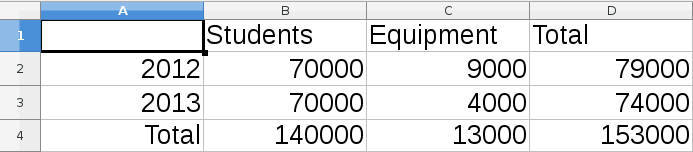
\includegraphics[scale=0.5]{images/spreadsheet.png}
    \end{center}
\end{frame}

\begin{frame}[fragile]
    \frametitle{New interaction mode}
    \begin{center}
        \begin{tikzpicture}
            \matrix{
                % title row
                 &
                \node{Students\strut}; &
                \node{Equipment\strut}; &
                \node{Total\strut}; \\
                % 2012 row
                \node{2012}; &
                \node(2012-students){70000}; &
                \node(2012-equipment){\change<4>{9000}{18000}}; &
                \node(2012-total){\change<5>{79000}{88000}}; \\
                % 2013 row
                \node{2013}; &
                \node(2013-students){70000}; &
                \node(2013-equipment){\change<4>{4000}{8000}}; &
                \node(2013-total){\change<5>{74000}{78000}}; \\
                % total row
                \node{Total\strut}; &
                \node(total-students){\color<2>{gray}140000}; &
                \node(total-equipment){\change<3>{13000}{26000}}; &
                \node(total-total){\change<2>{153000}{166000}}; \\
            };
        \end{tikzpicture}
    \end{center}
    \uncover<7>{\ldots and this happens behind the scenes, too.}
\end{frame}

\begin{frame}
    \frametitle{Straw-man abstract model}
    For universe $U$, lens $\ell \in \hyperlens N$ has components
    \begin{align*}
        put &\in 2^N \to U^N \to U^N \\
        K &\in 2^{U^N}
    \end{align*}
    \pause
    Inputs are really inputs and consistency is restored.
    \begin{align*}
        put(S,f)|_S &= f|_S \\
        put(S,f) &\in K \\
        \uncover<3>{put(\emptyset,f) &= f}
    \end{align*}
    \uncover<3>{Synchronizing too often doesn't hurt.}
\end{frame}

\begin{frame}[fragile]
    \frametitle{Unsolvable updates}
    \begin{center}
        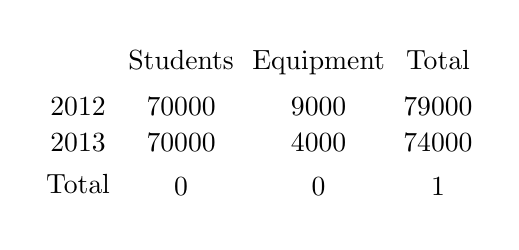
\begin{tikzpicture}
            \matrix{
                % title row
                 &
                \node{Students\strut}; &
                \node{Equipment\strut}; &
                \node{Total\strut}; \\
                % 2012 row
                \node{2012}; &
                \node(2012-students){70000}; &
                \node(2012-equipment){9000}; &
                \node(2012-total){79000}; \\
                % 2013 row
                \node{2013}; &
                \node(2013-students){70000}; &
                \node(2013-equipment){4000}; &
                \node(2013-total){74000}; \\
                % total row
                \node{Total\strut}; &
                \node(total-students){\alert{0}}; &
                \node(total-equipment){\alert{0}}; &
                \node(total-total){\alert{1}}; \\
            };
        \end{tikzpicture}
    \end{center}
    Track sets of names that are always solvable.
\end{frame}

\begin{frame}
    \frametitle{Composition intuition}
    \begin{center}
        \begin{tikzpicture}[node distance=3em]
            \uncover<+->{\draw
                node (center-top) {}
                node[replica,left of=center-top]       (Y-left-top)  {$Y$}
                node[lens,left of=Y-left-top]          (k-top)       {$k$}
                node[replica,left of=k-top]            (X-top)       {$X$}
                node[replica,right of=center-top]      (Y-right-top) {$Y$}
                node[lens,right of=Y-right-top]        (l-top)       {$\ell$}
                node[replica,right of=l-top]           (Z-top)       {$Z$}
                (X-top) -- (k-top) -- (Y-left-top)
                (Y-right-top) -- (l-top) -- (Z-top)
                ;
            }
            \uncover<+->{\draw
                node[replica,below of=center-top]      (Y-middle)    {$Y$}
                node[lens,left of=Y-middle]            (k-middle)    {$k$}
                node[replica,left of=k-middle]         (X-middle)    {$X$}
                node[lens,right of=Y-middle]           (l-middle)    {$\ell$}
                node[replica,right of=l-middle]        (Z-middle)    {$Z$}
                (X-middle) -- (k-middle) -- (Y-middle) -- (l-middle) -- (Z-middle)
                ;
            }
            \uncover<+->{\draw
                node[replica,below of=Y-middle]        (Y-bottom)    {$Y$}
                node[lens,below of=Y-bottom]           (kl-bottom)   {$k;\ell$}
                node[replica,left of=kl-bottom]  (X-bottom)    {$X$}
                node[replica,right of=kl-bottom] (Z-bottom)    {$Z$}
                (kl-bottom) -- (X-bottom)
                (kl-bottom) -- (Y-bottom)
                (kl-bottom) -- (Z-bottom)
                ;
            }
        \end{tikzpicture}
    \end{center}
    \uncover<3>{Safe updates: $\{X\}$ or $\{Z\}$.}
\end{frame}

\begin{frame}
    \frametitle{Ambiguous updates}
    \begin{center}
        \begin{tikzpicture}[node distance=3em]
            \draw
                node (center) {}

                node[replica,above left of=center]  (i1-left)  {\textrm I}
                node[replica,below left of=center]  (i2-left)  {$O_2$}
                node[lens,below left of=i1-left]    (k)        {$k$}
                node[replica,left of=k]             (o1)       {$O_1$}
                (k) -- (i1-left)
                (k) -- (i2-left)
                (k) -- (o1)

                node[replica,above right of=center] (i1-right) {\textrm I}
                node[replica,below right of=center] (i2-right) {$O_2$}
                node[lens,below right of=i1-right]  (l)        {$\ell$}
                node[replica,right of=l]            (o2)       {$O_3$}
                (l) -- (i1-right)
                (l) -- (i2-right)
                (l) -- (o2)

                node[below=3em of center]            (makes)     {$\Downarrow$}
                node[replica,below=0.2em of makes]   (i1-bottom) {\textrm I}
                node[lens,below of=i1-bottom]        (kl)        {$k;\ell$}
                node[replica,below left of=kl]       (o1-bottom) {$O_1$}
                node[replica,below of=kl]            (i2-bottom) {$O_2$}
                node[replica,below right of=kl]      (o2-bottom) {$O_3$}
                (kl) -- (i1-bottom)
                (kl) -- (i2-bottom)
                (kl) -- (o1-bottom)
                (kl) -- (o2-bottom)
                ;
        \end{tikzpicture}
    \end{center}
\end{frame}

\begin{frame}
    \frametitle{Two plans}
    \begin{center}
        \begin{tikzpicture}[node distance=3em]
            \path
                node[replica] (i1) {\textrm I}
                node[lens,below left of=i1] (k) {$k$}
                node[replica,below right of=k] (i2) {$O_2$}
                node[replica,left of=k] (o1) {$O_1$}
                node[lens,below right of=i1] (l) {$\ell$}
                node[replica,right of=l] (o2) {$O_3$}
                ;
            \draw[->] (i1) -- (k) ;
            \draw[->] (k)  -- (o1);
            \draw[->] (k)  -- (i2);
            \draw[->] (i1) -- (l) ;
            \draw[->] (i2) -- (l) ;
            \draw[->] (l)  -- (o2);
        \end{tikzpicture}
        \vfill
        \begin{tikzpicture}[node distance=3em]
            \path
                node[replica] (i1) {\textrm I}
                node[lens,below left of=i1] (k) {$k$}
                node[replica,below right of=k] (i2) {$O_2$}
                node[replica,left of=k] (o1) {$O_1$}
                node[lens,below right of=i1] (l) {$\ell$}
                node[replica,right of=l] (o2) {$O_3$}
                ;
            \draw[->] (i1) -- (l) ;
            \draw[->] (l)  -- (o2);
            \draw[->] (l)  -- (i2);
            \draw[->] (i1) -- (k) ;
            \draw[->] (i2) -- (k) ;
            \draw[->] (k)  -- (o1);
        \end{tikzpicture}
    \end{center}
    Observational equivalence is no help.
\end{frame}

\begin{frame}
    \frametitle{Remaining questions}
    \begin{itemize}
        \item Complete strategies for disambiguation?
        \item Behavioral specifications for disambiguation?
        \item How can we extend the static update check?
        \item What dynamic update checks are possible?
    \end{itemize}
\end{frame}

% TODO: how is the flow going to work? should it really go here, or earlier,
% or later, or... dunno lol
\begin{frame}
    \frametitle{Related work: bidirectional spreadsheets}
    \begin{itemize}
        \footnotesize
        \item Tiresias: The Database Oracle for How-To Queries

            \quad (Meliou and Suciu; SIGMOD ICMD 2012)
        \item A Spreadsheet Based on Constraints

            \quad (Stadelmann; UIST 1993)
        \item SkyBlue: A Multi-way Local Propagation Constraint Solver for
            User Interface Construction

            \quad (Sannella; UIST 1994)
        \item Expressing Multi-way Dataflow Constraint Systems as a
            Commutative Monoid Makes Many of their Properties Obvious

            \quad (J\" arvi, Haveraaen, Freeman, and Marcus; SIGPLAN WGP 2012)
        % TODO: read
        \item A Constraint-Based Spreadsheet for Cooperative Production
            Planning

            \quad (Chew and David; KBPPSC 1992)
        \item How to Use the Spreadsheet Manager

            \quad (Evans; tech report 1993)
        \item Interval Constraint Spreadsheets for Financial Planning

            \quad (Hyv\H onen; AIAWS 1991)
    \end{itemize}
\end{frame}

\nocollaborators
\section{Logistics}
\begin{frame}
    \frametitle{Timeline}
    \begin{center}
        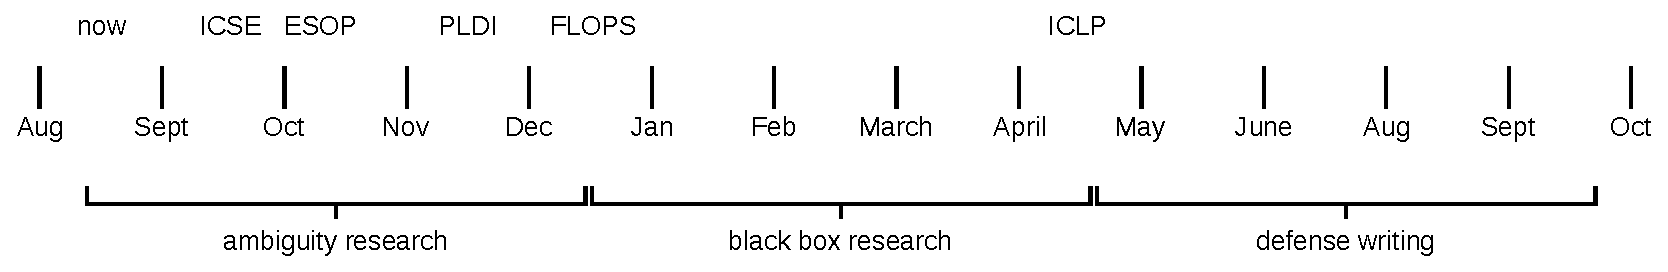
\includegraphics[scale=0.45]{timeline.pdf}
    \end{center}
    \begin{itemize}
        \item Nailing ambiguity resolution is lynchpin
        \item Extending static and dynamic checks is polish
        \item Bad case: trade black box time for additional ambiguity time
        \item Worst case: biased composition
    \end{itemize}
\end{frame}
% TODO: bonus slides on linear stuff?
\end{document}
